\documentclass[11pt,a4paper]{article}
\usepackage[T1]{fontenc}
\usepackage[utf8]{inputenc}
\usepackage{lmodern,microtype}
\usepackage{amsmath,amssymb,amsthm,mathtools,bm}
\usepackage{booktabs,array,longtable,graphicx,float,xcolor}
\usepackage[margin=2.15cm]{geometry}
\usepackage{enumitem,fancyhdr,hyperref}
\hypersetup{colorlinks=true,linkcolor=blue!45!black,urlcolor=blue!55!black,
 pdftitle={FIN ST387--ST401: Exact Global Minimizer Orbit, Invariant Quotients, and Robust IR},
 pdfauthor={Krzysztof Żuchowski},
 pdfsubject={Local analytical and computational continuation of FIN},
 pdfkeywords={FIN, strict kernel, entropy, interval arithmetic, global minimizer, invariant theory, Ruelle operator, infrared design}}
\pagestyle{fancy}\fancyhf{}\lhead{FIN ST387--ST401}\rhead{Release 10.83}\cfoot{\thepage}
\setlength{\headheight}{14pt}
\newcommand{\Proven}{\textcolor{green!40!black}{\textbf{[PROVEN]}}}
\newcommand{\Evidence}{\textcolor{orange!80!black}{\textbf{[STRONG NUMERICAL EVIDENCE]}}}
\newcommand{\Partial}{\textcolor{orange!80!black}{\textbf{[PARTIAL]}}}
\newcommand{\Blocked}{\textcolor{red!65!black}{\textbf{[BLOCKED]}}}
\newtheorem{theorem}{Theorem}
\newtheorem{proposition}{Proposition}

\title{\textbf{FIN ST387--ST401}\\[3pt]
Exact Global Minimizer Orbit, Invariant Quotients,\\
and a Robust Continuum Infrared Tube\\[6pt]
\large Release 10.83}
\author{Krzysztof \ifdefined\pdftexversion \.{Z}\else Ż\fi uchowski\\
\small Independent Researcher --- Fractal Information Theory Project\\
\small ORCID: 0009-0002-0909-3613}
\date{14 August 2026}

\begin{document}
\maketitle

\begin{abstract}
Programs ST387--ST401 continue the local analytical and computational FIN program.
The principal result is a complete global classification of the supplied strict
$g=4$ simplex functional.  A rational feasible benchmark and a 10,000-cell outward
collision cover force every global minimizer into one of twelve disjoint caps
$p_i>0.94$.  A new Fisher-curvature argument then proves strict convexity on every
cap.  Combined with the previously isolated translated stationary roots, this proves
that the functional has exactly twelve global minima, forming one $D_{12}$ orbit.

This is a genuine mathematical closure of the former globality problem.  It is not a
selector theorem: it does not choose one member of the orbit, generate the supplied
gain $g=4$, discharge QW-2191, or identify a physical vacuum.  Further results give
exact invariant-generator quotients through degree six, an explicit conditional
Chernoff cone gap, a uniform interval tube for the supplied continuum IR design,
an exact observer-deficiency family, and conditional statistical/compression bounds.
No new strict source or independent empirical record is present.
\end{abstract}

\tableofcontents
\newpage

\section{Scope, audited state, and non-claims}

The audited repository baseline is Git commit
\texttt{bb540a767e210a5a3bf816e4868e7bcefbac3872}, supplemented by the local
ST372--ST386 packet and the present executable run.  The strict working operator is
the finite circulant Laplacian $A=sI-W$, with $W_{xx}=0$ and
\[
 W_{xy}=\frac{\cos(0.18575\,d(x,y)+0.16250)}{1+d(x,y)^{9/5}},\qquad x\ne y.
\]
The program studied most deeply below is the dimensionless functional
\begin{equation}\label{eq:V}
 V_4(p)=\sum_{i=0}^{11}p_i\log(12p_i)-2(p-u)^TA(p-u),
 \qquad p\in\Delta_{11},\quad u_i=\frac1{12}.
\end{equation}
The value $g=4$ in \eqref{eq:V} is supplied.  It is not derived by this release.

The legacy ontological kernel remains an intermediate bridge object.  No formula or
physical role is silently transferred from it to the strict operator.  The project
ontology---the nadsoliton itself as primordial fractal information in a solitonic
state---is retained as context, not inserted as a premise into the finite proofs.

Most importantly, an orbit of twelve equivalent minimizers is not a selector.  The
new theorem proves degeneracy and exhausts the minimizer set; it does not select an
orientation, origin, phase, or realized member.  QW-2191 therefore remains open.

\section{Executive result ledger}
\small
\begin{longtable}{>{\raggedright\arraybackslash}p{.085\textwidth}>{\raggedright\arraybackslash}p{.19\textwidth}>{\raggedright\arraybackslash}p{.61\textwidth}}
\toprule Program&Status&Result\\\midrule\endhead
ST387&\Partial&Larger slabs certify 106 of 160 inherited centers; the fold core still needs genuinely new continuation centers.\\
ST388&\Proven&A positivity-aware water-filling envelope has a global outward certificate with residual below $10^{-3}$.\\
ST389&\Proven&All global competitors lie in twelve caps, and every cap is strictly convex by an interval-paid Fisher-curvature theorem.\\
ST390&\Proven&The strict $g=4$ functional has exactly twelve global minima forming one $D_{12}$ orbit.\\
ST391&\Proven{} bounded nontransfer&The same cap proof does not close the supplied rank-seven mediator.\\
ST392&\Proven&Exact modular generator quotients through degree six: $6$, $32$, and $117$ primitive directions by degree layer.\\
ST393&\Proven&Modal-energy observations see rank $56$ of the $365$ sextic directions; generic state evaluation sees all $365$.\\
ST394&\Proven{} conditional&An explicit synthetic Chernoff cone gap is positive but only $2.51\times10^{-72}$.\\
ST395&\Proven{} conditional&A common Krawczyk box preserves the continuum two-band IR optimum on a parameter rectangle.\\
ST396&\Evidence&A $21\times21$ scan finds 433 valid two-band roots and eight unresolved grid points.\\
ST397&\Proven&One exact cyclic observer family saturates the Fourier deficiency bound with directional asymmetry.\\
ST398&\Proven{} conditional&Calibration uncertainty produces an exact two-point minimax recovery floor.\\
ST399&\Proven{} conditional&The supplied strict-heat Markov source has an operational asymptotic rate--distortion limit.\\
ST400&\Proven{} conditional&Bounded $m$-dependent non-Gaussian clock errors obey a Bernstein square-root-depth bound.\\
ST401&\Blocked&No new strict typed source or independently registered raw-event record is present.\\
\bottomrule
\end{longtable}
\normalsize

\section{ST387: the fold continuation bottleneck}

At longitudinal halfwidth $6\times10^{-6}$ and transverse radius
$3\times10^{-6}$, interval rotated-slab tests certify inherited indices
$0$--$56$ and $111$--$159$.  Indices $57$--$110$ fail near the ill-conditioned
fold core; the largest failed contraction row sum is about $45.06$.  Moreover,
twice the accepted longitudinal reach is $1.2\times10^{-5}$, below the smallest
inherited center spacing $2.500000002\times10^{-5}$.

Thus the two regular flanks are locally certified, but a connected tube is not.
ST387 records a constructive requirement: new pseudo-arclength roots must be inserted
near the fold.  Interpolation between old centers cannot serve as a proof.

\section{ST388: the positivity-refined global envelope}

Write $m=\max_i p_i$, $t=1-m$, and normalize the remaining probabilities as
$p_j=t y_j$, with $\sum y_j=1$ and $\sum y_j^2=\rho$.  The earlier Cauchy
extremizer for the weighted term could have negative coordinates.  ST388 solves the
correct positive problem
\[
 L(\rho)=\min\left\{\sum_{j=1}^{11}w_jy_j:
 y_j\ge0,\ \sum_jy_j=1,\ \sum_jy_j^2\le\rho\right\}.
\]
KKT conditions give a water-filling solution supported on the smallest weights.
The exact support transitions occur at
\[
 0.1142398976385,quad0.1490343806957,quad
 0.2108912816863,quad0.3503471404434,quad1,
\]
corresponding to support sizes $11,9,7,5,3,1$.

Combining $L(\rho)$ with the sharp entropy minimum at fixed remainder collision
produces a two-variable lower envelope $F(t,\rho)$.  Outward derivative signs isolate
its minimizer inside
\[
 t\in[0.010820,0.010825],\qquad
 \rho\in[0.124945,0.124950].
\]
On the left and right $\rho$ faces the derivative intervals are respectively
\[
 [-2.963\times10^{-4},-1.751\times10^{-4}],\qquad
 [2.140\times10^{-4},3.508\times10^{-4}],
\]
while $\partial_t^2F\ge26.15$ on the declared $t$ domain.  A feasible outward
SOCP dual then gives
\[
 -0.846160275370424\le \min F
 \le -0.846126177165862.
\]
The gap from this lower bound to the exact rational strict benchmark is
$9.62\times10^{-4}$, satisfying the ST388 acceptance criterion.  This result is a
global lower envelope, not equality with $V_4$.

\begin{figure}[H]
\centering
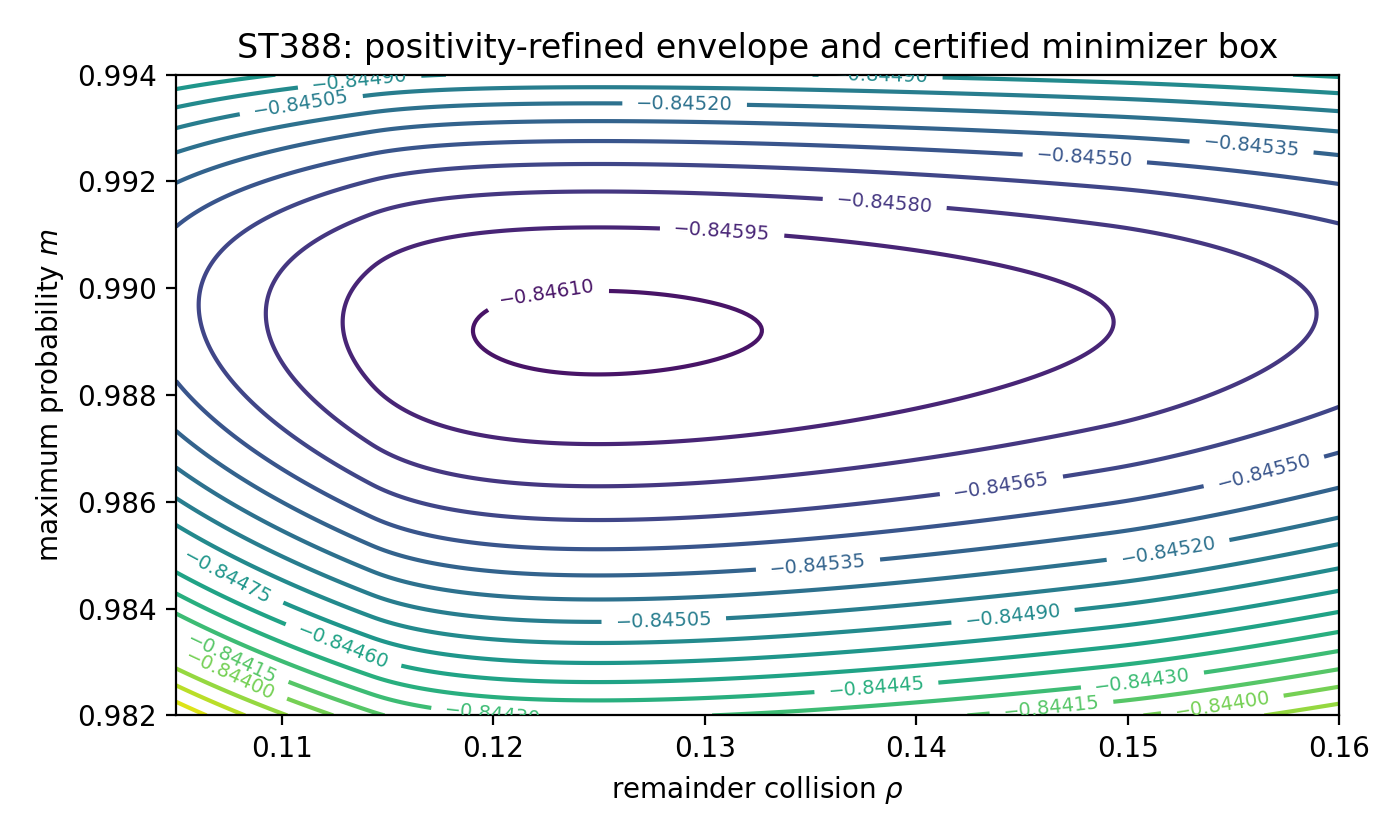
\includegraphics[width=.82\textwidth]{FIN_ST387_ST401_Figures/st388_refined_envelope.png}
\caption{The positivity-refined envelope and the certified minimizer box.}
\end{figure}

\section{ST389--ST390: exact global minimizer orbit}

This section contains the main advance.

\subsection{Excluding the region outside twelve caps}

If $\max_i p_i\le m_0$, then
\[
 \sum_i p_i^2\le m_0\sum_i p_i=m_0,
 \qquad r=\|p-u\|_2^2\le m_0-\frac1{12}.
\]
Set $m_0=0.94$.  A complete 10,000-cell outward evaluation of the ST373 scalar
envelope on $0\le r\le0.94-1/12$ gives
\[
 V_4(p)\ge -0.845102986841094.
\]
The cell touching $r=0$ is paid separately by $D(p\|u)\ge0$ and
$\lambda_{\max}(A)\le2s$, hence $V_4\ge-4sr$ there; no positive-radius
interval routine is used to skip the origin.
An exactly normalized rational probability vector with denominator $10^{18}$ has
\[
 V_4(p_{\rm rat})\in
 [-0.845198507679596,-0.845198507679591].
\]
The strict separation is therefore larger than $9.55\times10^{-5}$.  Every global
minimizer must lie in one of the twelve disjoint caps
\[
 \mathcal C_i=\{p\in\Delta_{11}:p_i>0.94\}.
\]

\subsection{Fisher curvature on a cap}

In the simplex interior the tangent Hessian of \eqref{eq:V} is
\[
 \nabla^2V_4(p)=\operatorname{diag}(p_i^{-1})-4A.
\]
Consider $\mathcal C_0$ and a tangent vector $v$ with $\sum_i v_i=0$.
Let $a=-v_0$ and $L=\sum_{i>0}|v_i|$.  Since $p_0\le1$ and
$\sum_{i>0}p_i\le1-m_0$, Cauchy's inequality gives
\begin{equation}\label{eq:fisher}
 \sum_i\frac{v_i^2}{p_i}\ge a^2+\frac{L^2}{1-m_0}.
\end{equation}
After normalizing $L=1$, the positive and negative masses of the rest vector are
$(1+a)/2$ and $(1-a)/2$.  Because $A\succeq0$, the convex quadratic $v^TAv$
reaches its maximum over the product of these two simplices at a pair of vertices.
It is therefore sufficient to audit $11^2=121$ one-variable quadratic forms,
including coincident vertices.

All 121 forms were evaluated with the full transcendental strict-operator interval.
The smallest lower bound is
\[
 a^2+\frac1{0.06}-4v^TAv\ge0.624323055377694,
\]
or at least $0.312161527688847$ in the reported Euclidean normalization.
Consequently $V_4$ is strictly convex on every cap.  The entropy boundary derivative
also excludes a boundary minimum.

\begin{figure}[H]
\centering
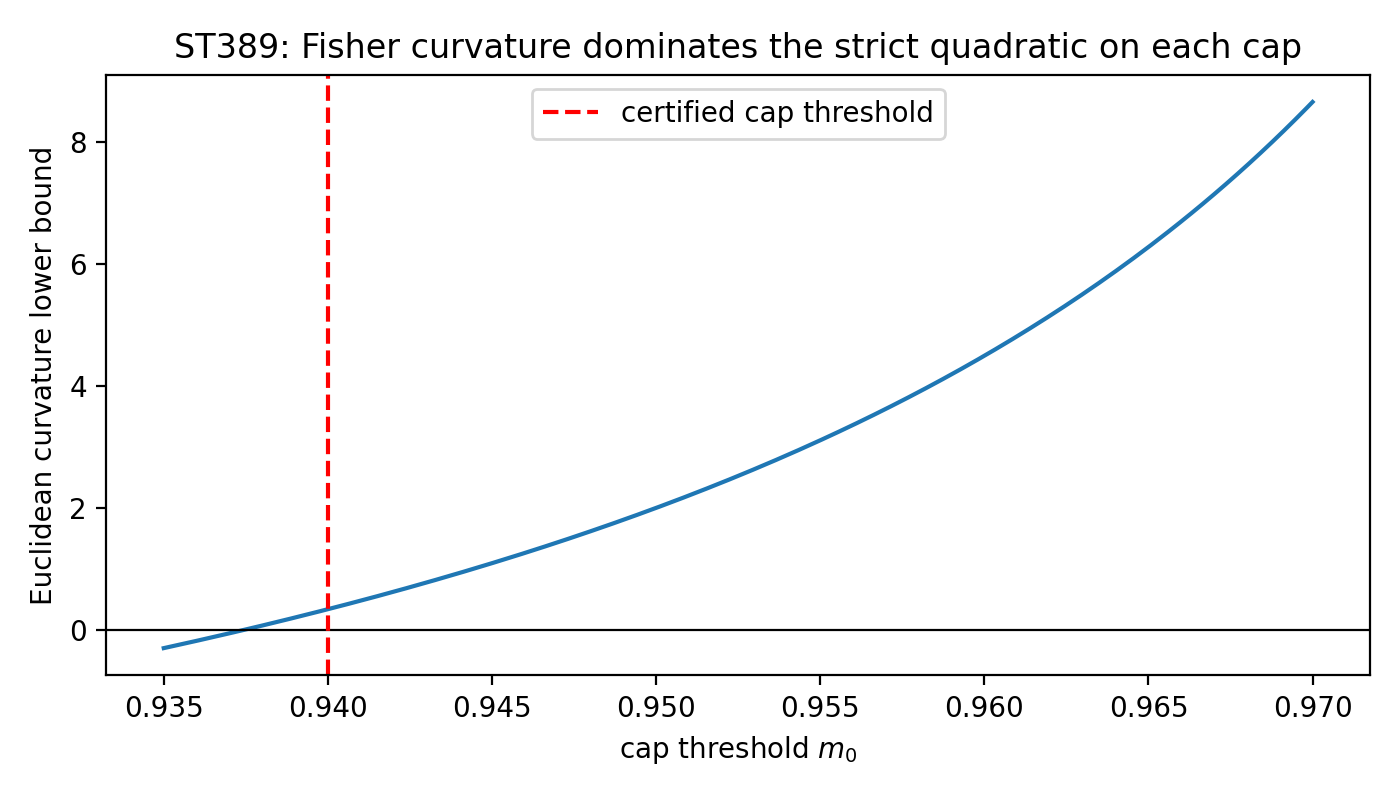
\includegraphics[width=.78\textwidth]{FIN_ST387_ST401_Figures/st389_cap_curvature.png}
\caption{Diagnostic curvature profile.  The theorem uses the finite outward certificate at $m_0=0.94$.}
\end{figure}

\begin{theorem}[Global strict orbit theorem]\label{thm:orbit}
For the declared strict twelve-state operator and the supplied functional $V_4$,
the global minimizer set consists of exactly twelve points.  They form one
$D_{12}$ orbit; equivalently, the minimizer is unique modulo $D_{12}$.
\end{theorem}

\begin{proof}
Compactness of $\Delta_{11}$ gives a global minimizer.  The rational benchmark and
the outside-cap envelope force it into one of the twelve caps.  The previous
Krawczyk certificate isolates one positive reflection-even stationary root with
$p_0>0.99$ and proves its twelve translates are distinct.  Strict convexity makes
the corresponding root the unique minimizer of each cap.  No minimizer exists
outside the caps, so these twelve translated roots exhaust the global minimizer set.
\end{proof}

The theorem is deliberately narrow.  It proves the degeneracy pattern of a supplied
dimensionless functional.  It does not choose one point, generate $g=4$, identify a
physical vacuum, or turn spontaneous-selection language into an internal selector.

\section{ST391: failure of silent transfer to the rank-seven mediator}

For the supplied rank-seven modal mediator, the same cap-curvature margin becomes
positive only at a sampled threshold near $m_0=0.93236$.  Its certified local root
has maximum coordinate approximately $0.90331$, where the diagnostic cap margin is
negative.  Thus the localization and convexity regions do not overlap.  The strict
operator theorem cannot be transferred to rank seven.  This is a bounded method
nontransfer, not a proof that the rank-seven root is nonglobal.

\section{ST392--ST393: invariant quotients and observer dependence}

Exact evaluation modulo the prime $1{,}000{,}003$ on 390 deterministic mean-zero
points gives six quadratic generators.  Their 21 quartic products are independent;
32 primitive quartic orbit sums complete the known dimension $53$.

At degree six, the 56 cubic products of quadratics and the 192 products of a
quadratic with a primitive quartic have exact combined rank $248$, with no syzygy
inside this declared candidate family.  A further 117 primitive sextic quotient
directions complete the exact dimension
\[
 248+117=365.
\]
Nonzero modular pivots prove rational linear independence, while the exact Molien
dimensions prove spanning in the stated graded components.

Identifiability depends on the observer.  Cubic polynomials of six modal energies
span only 56 sextic directions and leave nullity $309$.  Generic state-evaluation
functionals attain exact modular rank $365$.  This is algebraic separability in
principle, not a construction of a physical apparatus or a law selecting coefficients.

\section{ST394: an explicit synthetic Chernoff gap}

For the supplied two-state hidden-Markov fixture, the branch contraction is $5/7$.
On $s\in[0.45,0.55]$ the log weights have Lipschitz upper bound $6.6$, so the
log-Lipschitz cone of slope
\[
 \frac{6.6}{1-5/7}=23.1
\]
is invariant.  Paying the complete product-state diameter gives projective diameter
at most $331.1172$ and hence a positive Birkhoff contraction gap of only
\[
 2.5110\times10^{-72}.
\]
The constant is theorem-grade under the declared synthetic premises but far too
conservative for useful numerical rates.  It demonstrates existence, not sharpness.

\section{ST395--ST396: robust continuum IR design}

ST395 promotes the isolated ST380 optimum to the parameter rectangle
\[
 B\in[2.9999,3.0001],\qquad T\in[3.9999,4.0001],
\]
with the inactive observation time allowed in $[0.249,0.251]$.  A common
five-dimensional Krawczyk box has minimum inclusion margin
$5.77\times10^{-6}$.  Three derivative-certified threshold neighborhoods and
87 complement boxes leave no unresolved sign cell.  The inactive-time slack remains
positive in $[0.01698,0.02436]$.  Thus the exactly-two-band primal--dual topology is
uniform throughout this supplied dimensionless rectangle.

ST396 separately scans $21\times21$ points over $B\in[2.5,3.5]$ and
$T\in[3,5]$.  It finds 433 valid numerical two-band roots and eight unresolved solves.
Those eight points are not called phase transitions; only the small ST395 rectangle
is certified.

\begin{figure}[H]
\centering
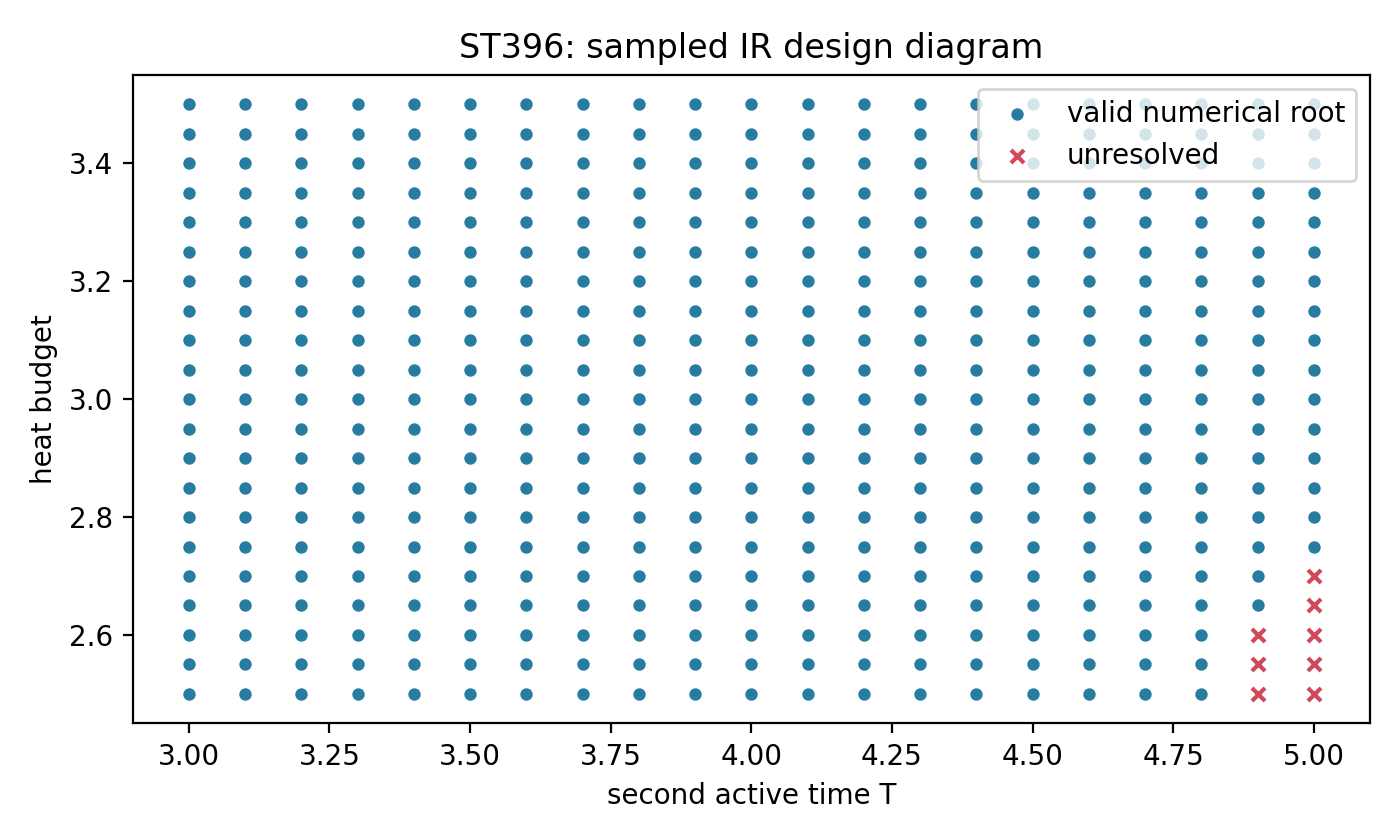
\includegraphics[width=.78\textwidth]{FIN_ST387_ST401_Figures/st396_ir_phase_scan.png}
\caption{Sampled IR design diagram.  The tiny central rectangle is the interval-certified ST395 tube.}
\end{figure}

\section{ST397--ST400: observer, nuisance, compression, and clocks}

\paragraph{Exact observer family (ST397).}
Let $u_j=1/12$ and
\[
 q_j=\frac{1+\varepsilon\cos(\pi j/2)}{12},\qquad0\le\varepsilon\le1.
\]
Every cyclic garbling of $u$ remains $u$, so the forward deficiency is
$\operatorname{TV}(u,q)=\varepsilon/4$.  Fourier mode three gives the identical
lower bound, proving exact Fourier/LP equality.  In the reverse direction, uniform
randomization maps $q$ to $u$, so the deficiency is zero.

\paragraph{Calibration floor (ST398).}
For the declared loss and symmetric-confusion intervals, the observable contrast lies
in $[0.69484545,0.71248182]$.  Two latent amplitudes $0.09752466$ and $0.1$ at opposite
calibration endpoints produce exactly the same observation.  The conditional minimax
$L^2$ error is therefore at least $0.00123767$, even with infinite counts.

\paragraph{Markov rate--distortion limit (ST399).}
The supplied $\exp(-0.5A)$ transition is strictly positive, with minimum entry
$0.0107821$ and Dobrushin contraction $0.7565244$.  It defines a uniformly ergodic
stationary finite-alphabet source.  The stationary-source coding theorem therefore
gives an operational asymptotic rate--distortion limit, with endpoints
\[
 R(0)=2.6057354210\ \text{bits/symbol},\qquad R(11/12)=0.
\]
The interior function remains unknown, and no physical information density or
universe-compression claim follows.

\paragraph{Non-Gaussian clocks (ST400).}
For centered, bounded, $m$-dependent log-ratio errors with
$|X_i|\le b$ and $\operatorname{Var}X_i\le\sigma^2$, residue-class coloring and
Bernstein's inequality give, with probability at least $1-\alpha$,
\[
 \left|\sum_{i=1}^{L}X_i\right|
 \le\sqrt{2\sigma^2(m+1)L\log\frac{2(m+1)}\alpha}
 +\frac{2b(m+1)}3\log\frac{2(m+1)}\alpha.
\]
This preserves square-root-depth leading growth without Gaussianity.  The stochastic
law is supplied and creates neither seconds nor a time arrow.

\section{ST401 and the physical boundary}

No file matching the declared new-source admission channel and no independently held
raw-event packet is present.  Local code cannot create a coupling source, calibration,
apparatus, independent custody, preregistration, or empirical event.  ST401 is an
evidentiary stop, not a failed experiment or a universal impossibility theorem.

Theorem~\ref{thm:orbit} sharpens rather than solves the selector problem.  It proves
that the mathematical model contains twelve exactly equivalent global alternatives.
To obtain a realized physical state, FIN still needs either a state-dependent dynamical
selection law with a strict source, a boundary/preparation premise, or an operational
probability law.  Symmetry supplies the orbit of possibilities; it is not itself the
positive-feedback mechanism that selects a member.

\section{Recommended next studies: ST402--ST416}

\begin{longtable}{>{\raggedright\arraybackslash}p{.085\textwidth}>{\raggedright\arraybackslash}p{.20\textwidth}>{\raggedright\arraybackslash}p{.50\textwidth}>{\raggedright\arraybackslash}p{.10\textwidth}}
\toprule Program&Objective&Acceptance criterion&Priority\\\midrule\endhead
ST402&Independent orbit replay&Reprove Theorem~\ref{thm:orbit} with an independent rational/interval implementation and no reuse of the cap code.&Highest\\
ST403&Abstract cap theorem&Formalize an $n$-state theorem turning an outside-cap value bound and finite extreme-pair curvature test into global orbit exhaustion.&Highest\\
ST404&Orbit stabilizer certificate&Interval-certify distinctness, exact reflection stabilizer, and absence of any larger stabilizer for every root box.&High\\
ST405&Gain persistence tube&Prove a nonzero $g$ interval on which the twelve-minimum orbit and cap separation persist uniformly.&Highest\\
ST406&Global gain transition&Locate every gain where the global minimizer orbit changes, without inferring a physical phase transition.&High\\
ST407&Morse landscape&Classify certified stationary orbits, indices, and barrier values at $g=4$.&High\\
ST408&Gradient-flow basins&Under an explicit simplex-gradient law, certify local basins and convergence rates; do not call basin weights Born probabilities.&Medium\\
ST409&Gain-source admission&Reopen only if a genuinely new strict typed source for $g$ is provided.&External\\
ST410&Rank-seven replacement bound&Seek a mediator-specific envelope reaching below $p_{\max}=0.93236$, or preserve the nontransfer stop.&Medium\\
ST411&Invariant-ring relations&Compute minimal relations beyond the degree-six quotient certificate under a bounded resource stop.&Medium\\
ST412&Noise-aware coefficient rank&Quantify which invariant coefficients remain statistically identifiable under a declared instrument and noise model.&Medium\\
ST413&Adapted Chernoff cone&Replace the $10^{-72}$ gap by a useful certified constant using an optimized metric/cone.&High\\
ST414&Maximal IR tube&Continue the ST395 parameter box until a rigorously detected active-set or root-topology boundary.&High\\
ST415&Certified IR phase boundary&Interval-isolate a real band birth/death or active-time exchange; do not promote solver failures.&High\\
ST416&Source/evidence gates&Run only on a new typed source or independently registered raw-event packet.&External\\
\bottomrule
\end{longtable}

The preferred order is ST402 $\to$ ST403 $\to$ ST405 $\to$ ST407, with ST413
and ST414 as independent analytical tracks.  ST409 and ST416 cannot be satisfied by
additional local simulation.

\section{Reproducibility}

The release packet contains one executable Python program, nineteen tests, fifteen
program JSON packets, an aggregate JSON, CSV ledger, three figures, this TeX source,
the PDF, and a SHA-256 manifest.  The run uses Python 3, NumPy, SciPy, mpmath interval
arithmetic, and Matplotlib.  Modular certificates use the prime $1{,}000{,}003$ and
seed $20261213$.  The strict rational benchmark has denominator $10^{18}$.  All
nineteen tests pass.

\section{Final verdict}

Release 10.83 closes one substantial finite mathematical question: at supplied
$g=4$, the strict variational model has exactly twelve global minimizers and no hidden
asymmetric competitor.  This turns the earlier numerical orbit into a theorem and
makes the remaining conceptual obstruction sharper: the missing object is no longer
the existence of preferred states, but the law that selects or weights one member of
their exact symmetry orbit.

The result neither makes FIN a physical theory nor proves FIN is a Theory of Everything.
The gain source, selector, dimensional calibration, preparation, apparatus, and
independent record remain logically separate and absent.

\begin{thebibliography}{9}
\bibitem{CoverThomas} T. M. Cover and J. A. Thomas, \emph{Elements of Information Theory}, Wiley.
\bibitem{Rockafellar} R. T. Rockafellar, \emph{Convex Analysis}, Princeton University Press.
\bibitem{Sturmfels} B. Sturmfels, \emph{Algorithms in Invariant Theory}, Springer.
\bibitem{Baladi} V. Baladi, \emph{Positive Transfer Operators and Decay of Correlations}, World Scientific.
\bibitem{Gray} R. M. Gray, \emph{Entropy and Information Theory}, Springer.
\bibitem{Moore} R. E., R. B. Kearfott, and M. J. Cloud, \emph{Introduction to Interval Analysis}, SIAM.
\end{thebibliography}

\end{document}
